\section{Approach}
\label{Approach}
\subsection{Activity Description Model}
When expressing a business process in BPEL, we are essentially defining a composite relationship of existing services. In BPEL, the $<invoke>$ primitive is used to represent the common task that invoke a Web Service instance. Nevertheless, in WoT, such kind of direct service binding may lead to several limitations. Because device environment is changeable and devices with similar functionalities offer different services, the cost of maintaining the process specification is very high. 

In the context of intelligent charging pill, the capabilities of the devices are exactly the same, but the process definition cannot be shared. The invoke bindings of the process must be rewritten to adapt the service interface of different charging pill. 

To address such limitations, a more abstract and more generate workflow definition is a feasible solution. We propose an activity description model, to attach ontological description for the business activity. The model can be represented as a tuple, 
\begin{equation}
	{AD} = \textless\textbf{DM}, \textbf{IM}, \textbf{OM}, \textbf{BF}\textgreater
\end{equation}where \textbf{DM}, \textbf{IM}, \textbf{OM}, \textbf{BF} denote domain, input messages, output messages, and business functionalities. Domain represents the device environment of current activity. Input messages and output messages contain variables with identity and data type. Business functionalities are consist of several verb-object constructions, which describe the business activity from a resource and operation perspective. 

\begin{figure}[!t]
\centering
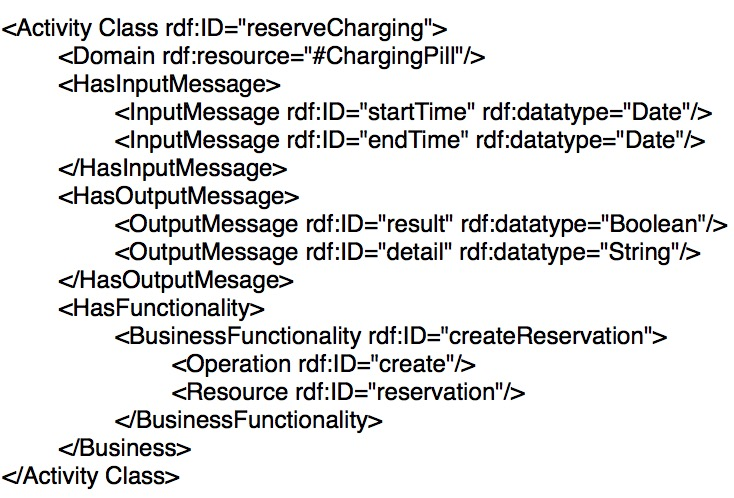
\includegraphics[width=1.0\linewidth]{./graph/activitydescriptionmodeldemo}
% where an .eps filename suffix will be assumed under latex, 
% and a .pdf suffix will be assumed for pdflatex; or what has been declared
%via \DeclareGraphicsExtensions.
\caption{Sample description of a reservation activity.}
\label{fig_activitydescriptionmodeldemo}
\end{figure}

In lots of semantic based service composition technologies, researchers perfer to take advantage of Input, Output, Pre-condition, Effect(IOPE) as the basis of service description and the critical parameters of the service matchmaking calculation\cite{syu2012survey}\cite{lee2013service}. However, in our model, we choose the simpler verb-object construction instead of the Pre-condition and Effect(PE), because: (1) Most of the RESTful Web Services in WoT are simple resource operations; (2) Defining a PE is much more sophisticated than defining a verb-object construction; (3) To campare with the semantic similarity calculation(between the functionality and the resource URL), the matchmaking calculation on PE is inefficiency. 

\begin{figure}[!b]
\centering
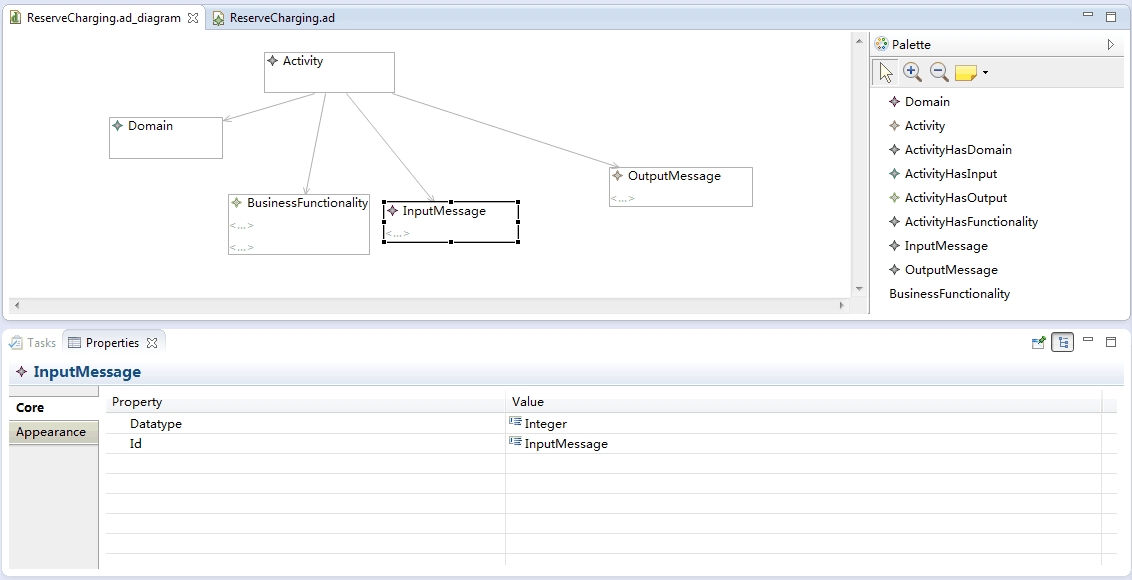
\includegraphics[width=1.0\linewidth]{./graph/eclipseplugin}
% where an .eps filename suffix will be assumed under latex, 
% and a .pdf suffix will be assumed for pdflatex; or what has been declared
%via \DeclareGraphicsExtensions.
\caption{A graphical modeling tool for the activity description model.}
\label{fig_eclipseplugin}
\end{figure}

Taking the charging pill as an example, an activity description model instance about the "reserveCharging" activity is shown in Fig.~\ref{fig_activitydescriptionmodeldemo}. The core resource operation of this activity is creating a reservation for a charging pill, which takes $startTime$ and $endTime$ as constructor arguments, and $result$ and $detail$ are returned to show whether the create operation is success or not and a detailed reason for the failure. 

Also, we try to provide a convenient and efficient way for users to specify their workflow in our model. As is shown in Fig.~\ref{fig_eclipseplugin}, a graphical modeling tool is afforded in the form of an Eclipse plugin. With such plugin, users can create an activity description model file for a business activity, drag and drop model nodes to the canvas, and fulfil the properties in an editing frame, just like defining a BPEL schema with the BPEL Designer for Eclipse. 

\begin{figure}[!t]
\centering
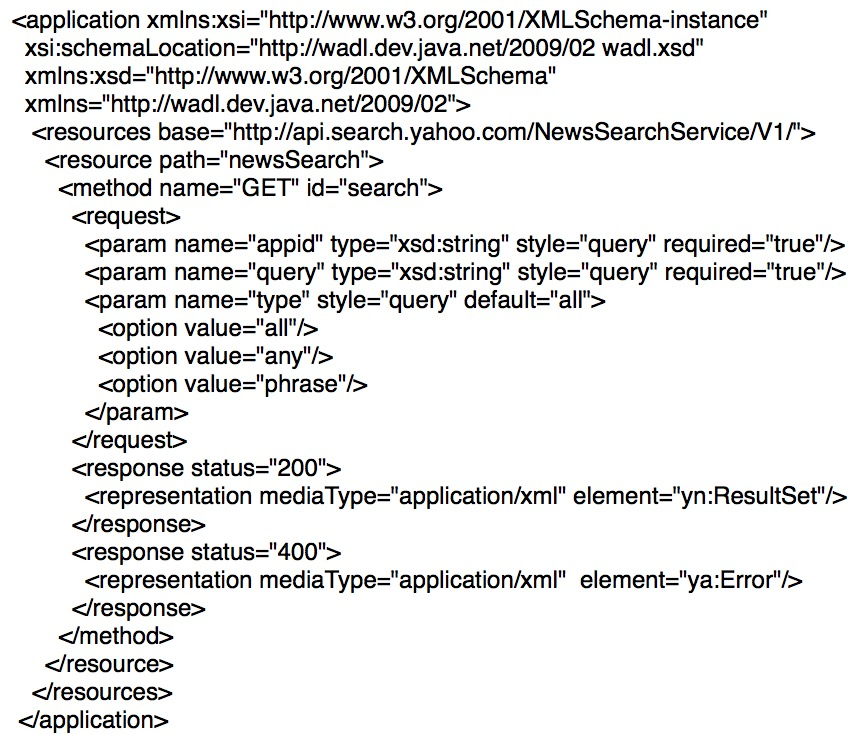
\includegraphics[width=1.0\linewidth]{./graph/wadl}
% where an .eps filename suffix will be assumed under latex, 
% and a .pdf suffix will be assumed for pdflatex; or what has been declared
%via \DeclareGraphicsExtensions.
\caption{Sample description of a reservation activity.}
\label{fig_wadl}
\end{figure}

\subsection{Matching Strategy}
In this subsection, we will give a detailed introduction to our matching strategy between our activity description model and device services. The WADL documents of those servics will be 
utilized for seeking out appropriate services that match the business functionality description. 

In actual Internet applications, capabilities provided by RESTful services are far more complex than pure resource operations, and the form of data exchange is more in nested structure like JSON and XML than basic data types like string or integer. But, as mentioned above, in the WOT environment, most RESTful services provided by smart devices are simple  resource operations, which will not be too complicated. Therefore, our matching strategy will pay more attention to the  equivalence of resources and operations, so that the complexity of the matching can be reduced to get a higher matching efficiency. 

Fig.~\ref{fig_wadl} shows a common WADL file example from Wikipedia. Generally speaking, a RESTful service denote an operation to a resource. Information about what resource the service has and how to invode the service is contained in the WADL document throught following nodes: (1) A $resources$ node is seen as a container for the $resource$ nodes, presenting the basic URL address of it's resources; (2) A $resource$ node specifies the resource to operate in the service with a path attribute; (3) A $method$ node is embodied in a $resource$ node to show the HTTP request method (e.g., GET, PUT, POST, DELETE) that can be accepted by the service, which also stand for the operation towards resource; (4) A $request$ node is a container for the $param$ nodes; (5) A $param$ node describes an input parameter of the service, including the data type of the parameter and whether such parameter is necessary or not. 

According to the WADL structure above, we can find that information about resource and operation of a service is in the $resource$ node and the $method$ node. In the $resource$ node, the path attribute is generally constitutive of a group of simple words, such as user/register and user/password/reset. Such group of words can always be divided into two part, a series of nouns to locate the URI of the resource, and a verb to appoint the operation on it. 

However, in some special cases, there might be no verb in a URL path. We often use a user/\{userid\}/orders  path to indicate the action that fetch all the orders of a user. In this circumstance, the operation information should be complemented by the HTTP request method in the $method$ node. There are eight HTTP request methods defined in the HTTP/1.1 specification, while the GET, PUT, POST, DELETE methods are the most commonly used ones. Owing to the HTTP specification, such methods have well known and dependable semantic meaning. A request with the GET method is always used for retrieving data. Consequently, for URL like user/\{userId\}/orders with the GET method, we can infer that it is a query service and the operation on the resource can be annotated as a "search" or a "get". Similarly, with a PUT or POST method, we can associate a "create" operation with a resource that have no specified identifier (e.g., userId), and an "update" operation with a resource that have specified identifier. 

After recognizing the resource and the operation of a service, we can refine the semantic similarity between the service and the business functionality defined in our activity description model. The similarity calculation formula is:
\begin{equation}
	Sim(f,s) = S(r_f,r_s) \times S(o_f,o_s)
\end{equation}
In (2), $f$ and $s$ denote the functionality(described in the model) and the service. $S(r_f,r_s)$ is the similarity between the resources in the functionality and the service, which can be predefined in an ontology repository or be retrieved in the WordNet\cite{wordnet}. 

Due to the limitation of performance in smart devices, we can assume that there will not be two services in one device that offer resemble operations on the same resource. Therefore, a conclusion can be drawn that the service with the highest similarity is the matching service. The algorithm for finding the matching service is defined in Algorithm~\ref{al_matching}. 
 \begin{algorithm}
        \caption{Find Matching Service}
        \begin{algorithmic}[1] 
            \Require resource and operation of a functionality description $R_f$, $O_f$, and services of a smart device $S = \{ s_1, s_2,\cdots,s_n\}$
            \Ensure the matching service to the functionality description
                   \For {each service $s_i$ in $S$}
                   	   \State Let $W_i$ be the WADL description of $s_i$
  					   \State Let $path$ be the path attribute of the resource node in $W_i$
  					   \State Split $path$ to get a word vector $WORD_i$
  					   \State Let $R_{si}$ and $O_{si}$ be the last noun and verb in the vector $WORD_i$
  					   \If {$O_{si}$ is null}
  					   		\State Complement the $O_{si}$ based on the $method$ node in $W_i$
  					   \EndIf
  					   \State $SIM_{si} \leftarrow Sim(R_f,R_{si}) \times Sim(O_f,O_{si})$ //$Sim(a,b)$ is the API to calculate the similarity between $a$ and $b$
				   \EndFor
				   \State Let $k$ be the index of the maximum similarity in $SIM$
				   \State\Return service $s_k$ 
        \end{algorithmic}
        \label{al_matching}
 \end{algorithm}
 
\begin{figure}[!t]
\centering
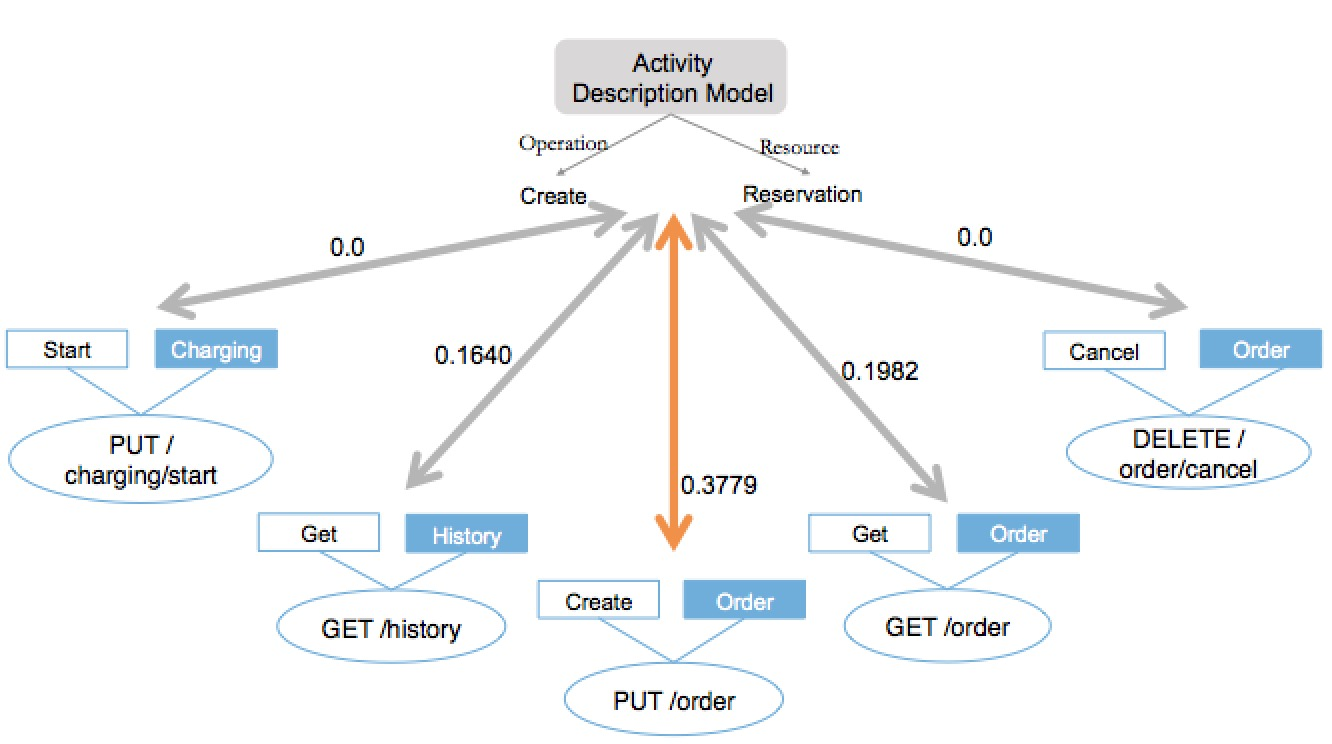
\includegraphics[width=1.0\linewidth]{./graph/matching}
% where an .eps filename suffix will be assumed under latex, 
% and a .pdf suffix will be assumed for pdflatex; or what has been declared
%via \DeclareGraphicsExtensions.
\caption{Matching result of a charging pile example.}
\label{fig_matching}
\end{figure}

A prototype application of the algorithm is implemented. Since there is no open colloction of WoT services to verify the precision of our matching, we have made a simple example for testing. Some RESTful services of the intelligent charging pile is obtained from an existing platform, and a matching result is shown in Fig.~\ref{fig_matching}. By using the WordNet, we calculate the similarity between five services and our functionality defined in Fig.~\ref{fig_activitydescriptionmodeldemo}. The "PUT /order" service is choosed to be the matching service because of the highest similarity, which is actually the operation to add a new reservation. However, there are several domain specified concepts that can not be retrieved in the WordNet, which may cause some wrong computing results. Therefore, a domain specified ontology repository is more suggested to optimize the matching accuracy. 

\subsection{General Service Model}
After the matching service is found, the following question arises:"How to generate a device-independent service with services on the device". 

An important factor to solve this question is to find the corresponding relation between the message description of the activity and the parameters of the services. For services with similar capabilities in various equipement environments, the form of passing arguments might be different. As an example, when querying for the same resource, the name and order of the query conditions might be different in different devices. 

Nevertheless, even if the representation is different, the data type and the semantic meaning of those parameters are consistent. Since the structures of the parameter description in our model and WADL are both consist of a name attribute and a data type attribute, the semantic based matching method is still a feasible solution. The semantic similarity calculation formula between two parameter descriptions is: 
\begin{equation}
    Sim(P_1, P_2)=
   \begin{cases}
   0 &\mbox{if $t_1$ and $t_2$ are not analogous}\\
   S(n_1, n_2) &\mbox{if $t_1$ and $t_2$ are analogous}
   \end{cases}
\end{equation}
where $t_1$ and $t_2$ are the data types of parameter description $P_1$ and $P_2$, and $n_1$ and $n_2$ are name of two parameters. A metrix can be predefined to check whether two data types are analogous(e.g., string and varchar are analogous but integer and date are not).

\begin{figure}[!b]
\centering
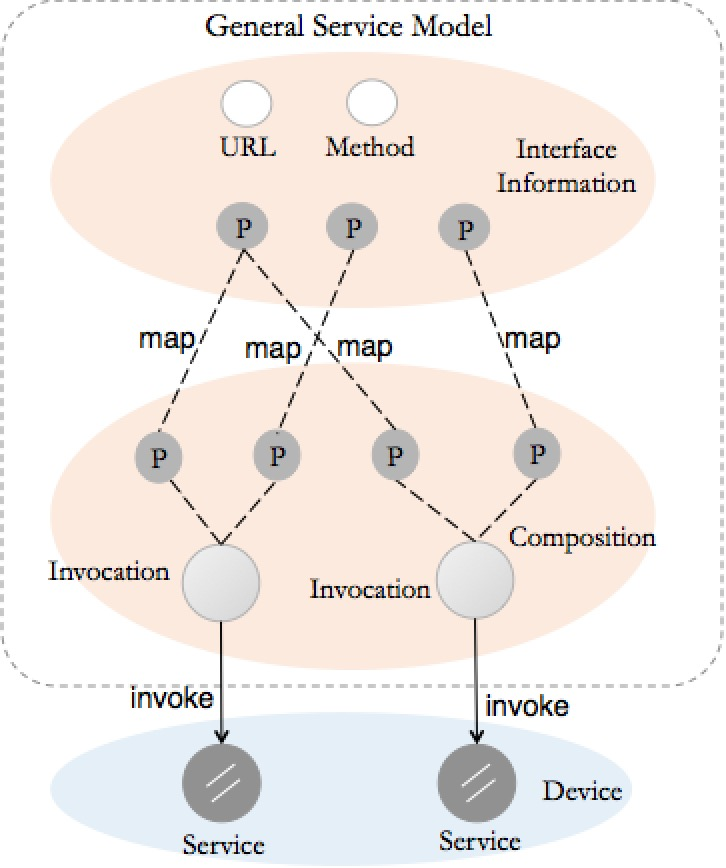
\includegraphics[width=1.0\linewidth]{./graph/generalservicemodel}
% where an .eps filename suffix will be assumed under latex, 
% and a .pdf suffix will be assumed for pdflatex; or what has been declared
%via \DeclareGraphicsExtensions.
\caption{Conception of the general service model.}
\label{fig_generalservice}
\end{figure}

As the matching degree of two parameter description is measured, we can now obtain the parameter matching result between our activity description and practical device services. 

In order to generate the device-independent service, we propose a general service model to express the composition of the services that match the business functionalities in an activity. 

A basic concept of the general service model is shown in fig.~\ref{fig_generalservice}. Structurally, the model is organized in two parts. The first part is the interface information of the general service, which defines the API for the composited service that fulfil the business activity. Considering the device-independency, the interface information is generated from the activity description model, including the URL path, the HTTP request method and the description of request and response parameters. The other one is the composition part. In this part, candidate services are listed with details about how to invoke the service and where to find the parameters. 

%generate the service code
 \begin{algorithm}
        \caption{Generate Service Code}
        \begin{algorithmic}[1] 
            \Require a general service model, including $URL$, $method$, input parameters $IP = \{ ip_1, ip_2,\cdots,ip_n\}$, output parameters $OP = \{ op_1, op_2,\cdots,op_n\}$ and invocations $Inv = \{ inv_1, inv_2,\cdots,inv_n\}$
            \Ensure source code of the service
            \State generate the service interface with $URL$ and $method$
            \For {each parameter $ip_i$ in $IP$}
            		\State set up the mapping between input $ip_i$ and content in $URL$
            \EndFor
            \For {each invocation $inv_i$ in $Inv$}
            		\State generate a new HTTP request with interface in $inv_i$ and parameters in $IP$
            		\State set up the mapping between output $OP$ and content in HTTP response
            \EndFor
            \State
            \Return the source code of the service
        \end{algorithmic}
        \label{al_generating}
 \end{algorithm}
 
Assume we need to execute an activity on two different devices. For each device, a general service model is generated. Comparing two models, we can find that the contents of their interface information part are exactly the same, to make the same HTTP request can be directly reused in both devices. On the contrary, the composition parts on two models are device specific, to composite the actual services on the device. 

Since the general service model furnish an abstract description about the service composition, the specific JavaScript code can be generated to implement and deploy the general service on a Node.js server\cite{wotframework}. A rough process for code generation is introduced in Algorithm~\ref{al_generating}. 

The general service provides a device-independent interface to decouple business code from specific device service. Business activity can bind with the general service instead of the original services on the device. When there is an replacement between two different devices, the process can switch to the new device without any modification about the source code. 



